\section{Introduction}
%\addcontentsline{toc}{chapter}{Introduction}
%\markboth{Introduction}{Introduction}

% Put your introduction here. You can reference other chapters, sections, images, etc.\ using the \texttt{cleveref} package like this:~\cref{ch:terminology}.

The study of \textit{snarks}, that is $2$-connected cubic graphs that are not 3-edge-colourable, is~important since they are smallest possible counterexamples for several open problems.
One such conjecture is the Cycle Double Cover Conjecture stating that each bridgeless graph has a family of cycles, such that each edge appears in exactly two of the cycles.
To exclude trivial cases, some additional properties are required from snarks like the following.

Let $G$ be a cubic graph and $S$ an edge-cut of size $n$. If at least two components of $G - S$ contain a cycle, $S$ is said to be an \textit{n-edge-c-cut}. Generally, these edge-cuts are called \textit{c-cuts}. 
A cubic graph $G$ is \textit{cyclically n-edge-connected} if there is no c-cut with less than $n$ edges. \textit{Cyclic edge-connectivity} of a cubic graph $G$ having at least one c-cut is the smallest number of edges of a c-cut of $G$.
Another measurement of nontriviality is the \textit{girth} of a graph $G$ which is the minimum length of a cycle in $G$. If $G$ does not contain a cycle, we set the girth to $\infty$.

Many authors (e.g. \cite{Preissmann1983, Nedela1996}) require that snarks have girth at least $5$ and are cyclically 4-edge-connected. We call such snarks \emph{non-trivial} and the remaining ones \emph{trivial}. On the other hand, some authors allow snarks to contain bridges \cite{IrreducibleSnarksSkoviera}. 
%making the dumbbell graph on two vertices the smallest snark (\cref{fig:dumbbell}).

%\begin{figure}
%	\centering
%	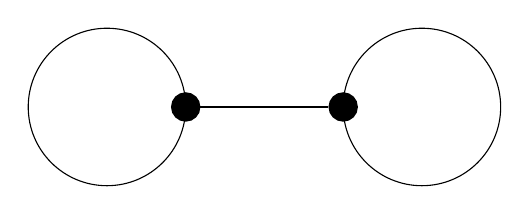
\begin{tikzpicture}[every node/.style={draw,circle,very thick, fill=black}]
	\node[shape=circle,draw=black] (1) at (0,0) {};
	\node[shape=circle,draw=black] (2) at (2,0) {};
	
	\path 
	(1) edge (2)
	;
	
	\draw (-1,0) circle [radius=1];
	\draw (3,0) circle [radius=1];
\end{tikzpicture}
%	\caption{Dumbbell graph}
%	\label{fig:dumbbell}
%\end{figure}

According to our definition, the Petersen graph (see \cref{fig:petersen}) is the smallest snark and it satisfies every definition of a snark. Other notable snarks are the Blanuša snarks \cite{Blanusa}, or the infinite family of flower snarks discovered by R. Isaacs \cite{Isaacs1975}. The Isaacs snarks are denoted by $J_k$, where $k$ is an odd integer $k\geq 3$.

\begin{figure}
	\centering
	\begin{tikzpicture}[every node/.style={draw,circle,very thick, fill=black}]
	\graph[clockwise, radius=2cm, empty nodes] {subgraph C_n [n=5,name=A] };
	\graph[clockwise, radius=1cm, empty nodes] {subgraph I_n [n=5,name=B] };
	
	\foreach \i [evaluate={\j=int(mod(\i+2+4,5)+1)}]% using Paul Gaborit's optimisation
	in {1,2,3,4,5}{
		\draw (A \i) -- (B \i);
		\draw (B \j) -- (B \i);
	}
\end{tikzpicture}
	\caption{Petersen graph}
	\label{fig:petersen}
\end{figure}

Determining whether a given graph is a snark is an NP-complete problem \cite{HolyerNP}. However, when creating a cubic graph from some smaller building blocks, of which we know their colouring properties, we also know the colouring properties of the result. This may also include if it is a snark or not. These building blocks are called multipoles (e.g. see \cite{Nedela1996}) and can be described as an extended type of a graph that allows dangling edges. Multipoles are useful for various constructions of snarks \cite{IrreducibleSnarksSkoviera,Lukotka15} or also for their structural analysis \cite{ChladnyFactorisation,MorphologyOfSmall}.

%TODO: tu by sa ešte zišlo možno ešte pár slov

%Each edge has two edge ends, which may or need not be incident with some vertex. If some edge is incident with only one vertex, we say it is \textit{dangling}. The edge ends not incident with any vertex are called \textit{semiedges}.

%Usually, multipoles are constructed from cubic graphs by removing some vertices or severing some edges. In our research, removing a vertex from a graph involves keeping the edges incident with the vertex but making them dangling. This means that the edge ends that were previously incident with the removed vertex are no longer incident with any vertex, thus resulting in a multipole. Similarly, severing an edge involves replacing it with two new dangling edges from its end vertices. Using these dangling edges, we can connect multiple multipoles to create bigger building blocks or even graphs. This means that the analysis of the colouring properties of these multipoles can aid in the study and construction of snarks.
%
%By talking about proper (2,3)-poles, we mean a specific type of a multipole with five dangling edges (usually named a 5-pole), for which we can divide the semiedges into two so-called connectors, one with two semiedges and one with three. Also, they fulfil the condition of being proper (\cref{sec:multipole-colouring}). In general, by $k$-poles, we denote multipoles that have exactly $k$ semiedges. Proper (2,3)-poles can be created by removing a vertex from a snark and severing one edge.

%Exploring multipoles effectively involves starting with the simplest ones and gradually moving towards more complex ones. That's why we have chosen to investigate the $k$-poles starting with the smallest value of $k$. The reason we are exploring 5-poles is that for each $k<5$, the colourability of $k$-poles has already been investigated. Specifically, the colouring properties of 1-poles, 2-poles, and 3-poles are trivial, and the colouring properties of 4-poles are limited and have already been sufficiently explored.

%It can be proven that if we get two 3-edge-colourable 5-poles by severing five edges in a given snark, they can be only one of three types: negators, superpentagons and proper $(2,3)$-poles. The colouring properties of the first two are known, only the last type of 5-poles still needs to be explored, and thus we want to shed some light on them as~well.

%Our work analyses the colouring properties of proper (2,3)-poles originating from small snarks. Based on the analysis results, we then formulate propositions on sufficient and necessary conditions on the colouring properties of proper (2,3)-poles. 

%This thesis is structured as follows: In \cref{ch:multipoles-and-snarks}, we define and explain the terms necessary for understanding this topic, like the mentioned snarks, multipoles and others. In \cref{ch:proper-23-poles}, we explain what the~proper (2,3)-poles are. We define the mentioned colouring properties and divide proper (2,3)-poles into classes based on their colouring properties. In \cref{ch:our-work}, we present the~results of our work. To begin, we explain the methods of analysis we used, including a~simplified explanation of the algorithm and the format of the~outputs. We also provide some multipoles that can modify the colouring properties of proper (2,3)-poles. The~following section comprises the core of our work, presenting the theorems regarding the~colouring properties of proper (2,3)-poles. Specifically, we explore the necessary and sufficient conditions for these properties. Lastly, we provide data and observations from our analysis, including problems and questions that arose while exploring proper (2,3)-poles. We answer some of them but also include unanswered questions and problems that can be explored in further research.

This paper is structured as follows. First, we develop the theory needed for our work. In \cref{sec:multipoles}, we define multipoles and all notions related to them, and in \cref{sec:multipole-colouring}, we develop the theory for describing colouring properties of multipoles. \cref{sec:5-poles} is specifically devoted to multipoles with five dangling edges while it explains the relation of proper (2,3)-poles to them. In \cref{ch:proper-23-poles}, we introduce several classes of proper (2,3)-poles with respect to their colouring properties. The rest of the paper focuses on our results. \cref{sec:analysis} describes methods of our computer-assisted analysis of proper (2,3)-poles constructed from small non-trivial snarks. In \cref{sec:classes-to-perfect}, we provide multipoles that can be used to change colouring classes of proper (2,3)-poles. \cref{sec:result-theorems} contains theoretical results on colouring properties of proper (2,3)-poles. At the end, in \cref{sec:observations}, we summarise the results of our computer-assisted analysis.

Definitions not provided in our work can be found in the book \quotes{Graph Theory} by R. Diestel \cite{Diestel2010}.
We only clarify that all graphs considered in this work are undirected, and while we permit multiple edges, loops are not allowed. 
The distance between two vertices $x$ and $y$ in a graph $G$, denoted by $d_G(x,y)$, is defined as the length of a shortest path between $x$ and $y$ in $G$. If no such path exists, we set $d_G(x,y)=\infty$. The distance $d_G(x, ab)$ between a vertex $x$ and an edge $ab$ is defined as the~smallest value between $d_G(x,a)$ and $d_G(x,b)$.
